\documentclass{article}
\usepackage{url,amsfonts, amsmath, amssymb, amsthm, graphicx, braket, fancyhdr, physics, mathtools, hyperref}
% Change this path if you use images
\graphicspath{ {./Classical_Images/} }
% Page layout
\setlength{\textheight}{8.75in}
\setlength{\columnsep}{2.0pc}
\setlength{\textwidth}{6.5in}
\setlength{\topmargin}{0in}
\setlength{\headheight}{0.0in}
\setlength{\headsep}{0.0in}
\setlength{\oddsidemargin}{0in}
\setlength{\evensidemargin}{0in}
\setlength{\parindent}{1pc}

% Commands
\newcommand{\RNum}[1]{\uppercase\expandafter{\romannumeral #1\relax}}
\newcommand{\Lagr}{\mathcal{L}} % Lagrangian
\newcommand{\vcurl}[1]{\vec{\nabla}\times \vec{#1}} % Curl with vector notation
\newcommand{\fhalf}{\frac{1}{2}} % 1/2 fraction
% Shortcut for general Euler-Lagrange Equation
\newcommand{\EulLagreq}{\dv{}{t} \left( \pdv{ \Lagr}{\dot{x_i}} \right) &= \pdv{\Lagr}{x_i}}
% Trig Shorts
\newcommand{\sinth}{\sin{\theta}}
\newcommand{\costh}{\cos{\theta}}
\newcommand{\cotth}{\cot{\theta}}
\newcommand{\tanth}{\tan{\theta}}
\newcommand{\cscth}{\csc{\theta}}
\newcommand{\secth}{\sec{\theta}}

\usepackage[a4paper,margin=2.5cm,portrait, headsep=24pt, headheight=2cm]{geometry}
\usepackage{enumitem}

% Header
\pagestyle{fancy}
\fancyhf{}
\rhead{Page \thepage}
\chead{Classical Mechanics DE}
\lhead{James Natoli}
\rfoot{}

\begin{document}
% suppress header on first page
\thispagestyle{empty}
%%% Title Stuff
\begin{center}\Large \textbf{Classical Mechanics Departmental Exam} \\
\normalsize James Natoli \\  January 2021
\end{center}

%%%%%%%%%%%%%%%%% Problem 1 %%%%%%%%%%%%%%%%%
\section*{Problem 1} 
% Problem Statement
Consider a planet in a circular orbit around a star. Determine how the speed of the planet depends on how far away it is from the star. Does Pluto move faster or slower than Mercury around the run?
%% Solution Here
\section*{\textit{Solution}} 
Let's start with centripetal force, $ F_c = \frac{mv^2}{r}$ and gravitational force, $F_g = G\frac{Mm}{r^2}$
As these are the only forces, we can set them equal to each other and work from there
\begin{align}
\frac{mv^2}{r} &= G\frac{Mm}{r^2} \\
v^2 &= \frac{GM}{r} \\
v &= \sqrt{\frac{GM}{r}} \\
v &\propto \frac{1}{\sqrt{r}} 
\end{align}
So because velocity depends on $ \frac{1}{\sqrt{r}}$, \boxed{\text{Pluto will move slower than Mercury}}
%%%%%%%%%%%%%%%%% Problem 2 %%%%%%%%%%%%%%%%%
\section*{Problem 2} 
% Problem Statement
A satellite in circular orbit of radius R about the center of the earth is subject to a drag force of magnitude $F = av^n$ (where $v$ is the speed of the satellite) which results in the rate of change of the radial distance $\frac{dr}{dt} = -b$ (where $b > 0$ is small enough so that the loss of energy in an orbit is small compared to the total kinetic energy of the satellite). Determine $a$ and $n$
%% Solution Here
\section*{\textit{Solution}} 
Start with the Virial Theorem, which states that the average kinetic energy is equal to minus one half of the average potential energy, or
\[ T_{avg} = -\frac{1}{2}V_{avg} \]
In circular orbits, $ T_{avg} =T$ and $V_{avg} = V$
\begin{align}
	E = T + V &= -\frac{1}{2}V + V = \frac{1}{2}V \\ 
	\text{where gravitational potential is }V &= -\frac{GMm}{r} \\ 
	E &= -\frac{GMm}{2r} 
\end{align}
Next, we have to find a way to get some derivatives, because the problem gives us $\frac{dr}{dt} = -b$
\begin{align}
	dW = E &= \vec{F} \cdot \vec{x} \\
	\frac{dE}{dt} &= \vec{F} \cdot \frac{d\vec{x}}{dt} \\  
	\frac{dE}{dt} &= \vec{F} \cdot \vec{v} \\ 
	\text{and using (7), }& \\
	\frac{dE}{dt} &= \frac{GMm}{2r^2} \dot{r} \\ 
	\text{now use }& \dot{r} = -b, \\ 
	\frac{dE}{dt} &= -\frac{GMm}{2r^2} b
\end{align}
We also know that $\vec{F} \cdot \vec{v} = -av^n \cdot v = -av^{n+1}$, where this is negative because drag force is always opposite the direction of motion
Also recall from circular orbits (or the previous problem) that when we set centripetal force = gravitational force, we get $v = \sqrt{\frac{GM}{r}}$, so this leaves us with
\[ \vec{F} \cdot \vec{v} = -a\left(\frac{Gm}{r}\right)^\frac{n+1}{2} \]
Now use this (above) combined with (10) and (7) to get
\[ -\frac{GMm}{2r^2}b = -a\left(\frac{Gm}{r}\right)^\frac{n+1}{2} \]
To find a and n, we can set $n = 1$
\[ \frac{GMm}{2r^2}b = a\frac{GM}{r} \]
\[\boxed{a = \frac{mb}{2r}} \]
I suppose you could find $a$ for other values or $n$, or solve them for each other, but this was about as far as I felt like going 

%%%%%%%%%%%%%%%%% Problem 3 %%%%%%%%%%%%%%%%%
\section*{Problem 3 } 
% Problem Statement
Consider a mass m in a circular orbit of radius R in a central-force potential $-am/r^n,a>0$. Determine the range of $n>0$ for which such a circular orbit is stable
%% Solution Here
\section*{\textit{Solution}} 
Alrighty, let's first recall the condition for stability. As far as mental stability goes, I'm in the dark, but for orbital stability we require that the second spatial derivative of the effective potential is $>$ 0
\[ \frac{d^2V_{eff}}{dr^2} > 0\]
where the effective potential is, $V_{eff} = V + \frac{l^2}{2mr^2}$
\begin{align}
	\frac{dV_{eff}}{dr} = \frac{d}{dr}\left(\frac{l^2}{2mr^2} - \frac{am}{r^n}\right) &= 0 \\ 
	= -\frac{l^2}{mr^3} + \frac{anm}{r^{n+1}} &= 0 \\ 
	\frac{l^2}{mr^3} &= \frac{anm}{r^{n+1}} \\ 
	\frac{d^2V_{eff}}{d^2r} = \frac{d}{dr}\left( -\frac{l^2}{mr^3} + \frac{anm}{r^{n+1}}\right) &> 0 \\
	\frac{3l^2}{mr^4} - \frac{(n+1)nam}{r^{n+2}} &> 0 \\ 
	\frac{3}{r} \left(\frac{l^2}{mr^3}\right) - \frac{(n+1)nam}{r^{n+2}} &> 0 \\
	\text{now we use (17), } \frac{3}{r} \left(\frac{nam}{r^{n+1}}\right) - \frac{(n+1)nam}{r^{n+2}} &> 0 \\
	3 \left(\frac{nam}{r^{n+2}}\right) - (n+1) \left( \frac{nam}{r^{n+2}} \right) &> 0 \\
	3 - (n+1) &> 0 \\
	2 &> n
\end{align}
And so, \boxed{n < 2} in order for the orbit to be stable \\
\\
Note: I'm not exactly sure why we set the original first derivative to 0, maybe because we're looking at the potential minimum

%%%%%%%%%%%%%%%%% Problem 4 %%%%%%%%%%%%%%%%%
\section*{Problem 4} 
% Problem Statement
The gravitational acceleration on the surface of the moon is one-sixth of that on the surface of the earth. A woman on Earth lowers her center of mass by 40 cm by bending her knees. Exerting a constant force on the ground, she jumps straight up, raising her center of mass by 60 cm above that of her normal erect position. How much higher can she jump on the moon?
%% Solution Here
\section*{\textit{Solution}} 
First, let's establish that $\Delta h_{earth} = 1.0$ m. She also applies the same force both times, over the same distance, so we can also say that $W_{Earth} = W_{Moon}$
\begin{align}
	W_{Earth} &= V_{final} - V_{initial} \\
	&= mgh_f - mgh_i \\ 
	&= mg(\Delta h_{earth})
\end{align}
We also have the following expression for the moon's work
\[ W_{Moon} = m \left( \frac{g}{6} \right) \Delta h_{Moon} \]
Now, let's set these 2 work expressions equal to eachother...
\begin{align}
	W_{Moon} &= W_{earth} \\ 
	m \left( \frac{g}{6} \right) \Delta h_{Moon} &= mg(\Delta h_{earth}) \\
	\Delta h_{Moon} &= 6 \Delta h_{earth}
\end{align}
So she can jump \boxed{\text{ six times higher}} than on Earth

%%%%%%%%%%%%%%%%% Problem 5 %%%%%%%%%%%%%%%%%
\section*{Problem 5} 
% Problem Statement
A uniform rigid rod of length L, mass m, and moment of inertia $mL^2/3$ about an end, is supported horizontally by props at each end. Find the force at the second prop right after the first one is removed.
%% Solution Here
\section*{\textit{Solution}} 
This problem was a little difficult for me to visualize, so I've included a picture
\begin{figure}[h]
	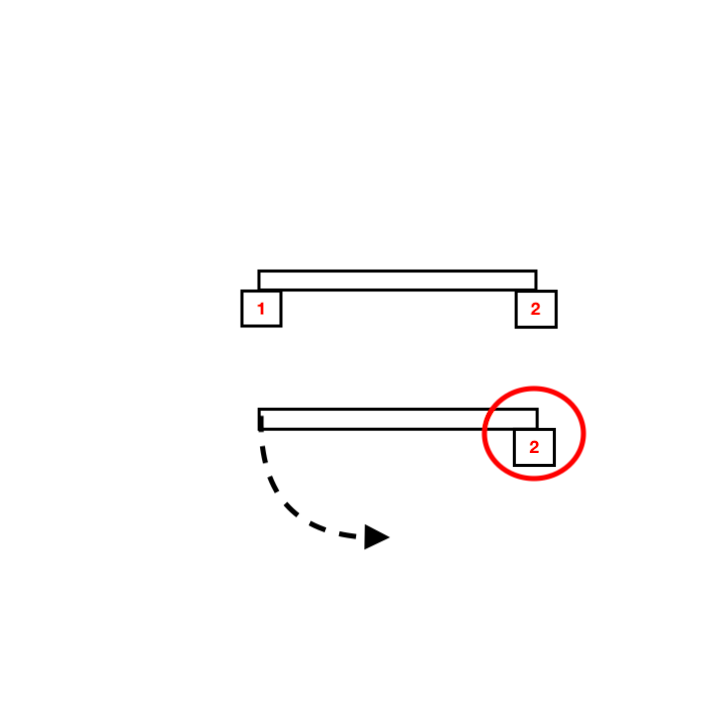
\includegraphics[scale=0.5]{P5}
	\centering
\end{figure}
Here, we can see the support on the left has been removed, allowing the rod to swing down. We are focusing on the force on the support on the right the moment it is removed. Let's start with a free-body diagram. In lieu of drawing it, we can see that there are only 2 forces involved, gravity pulling the bar down and acting on its center of mass, and the force from the support, pushing back up. 
\[ \Sigma F_y = mg - F_s = ma_y \]
Where $a_y$ is acceleration in the y direction and $F_s$ is the support force, what we are solving for
\[ F_s = mg - ma_y \]
We also need to consider Torques, because the gravitational force is acting at the center of mass, not the point of rotation. Lets state the same law but for Torques
\begin{align}
	\Sigma \tau = I \ddot{\theta} &= \vec{r} \times \vec{F_g} \\
	\frac{mL^2}{3} \ddot{\theta} &= \frac{L}{2} \cdot mg \\
	\ddot{\theta} &= \frac{3g}{2L}
\end{align}
In (29) the cross product simplifies to multiplication because the radial vector is perpendicular to $F_g$, and $r = \frac{L}{2}$ because that is the distance to the center of mass, the midpoint of the rod \\ \\ 

Now, we use some angular to linear conversions, listed below
\begin{align}
	v_y &= r\dot{\theta} \\
	a_y &= r\ddot{\theta} \\
	r &= \frac{L}{2}
\end{align}

Now let's put (32) - (34) together with $ F_s = mg - ma_y $ and solve

\begin{align}
	F_s &= mg - ma_y \\ 
	&= mg - m\left( \frac{L}{2} \right) \left( \frac{3g}{2L} \right) \\
	&= mg - \frac{3mg}{4} \\ 
	&= \frac{mg}{4}
\end{align}
And so \boxed{F_s = \frac{mg}{4}} at the moment the first support is released

%%%%%%%%%%%%%%%%% Problem 6 %%%%%%%%%%%%%%%%%
\section*{Problem 6} 
% Problem Statement
Consider two identical masses m and two identical springs of spring constant k and unstretched length a.
\begin{figure}[h]
	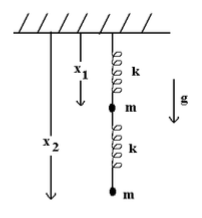
\includegraphics[scale=0.5]{P6}
	\centering
\end{figure}
\begin{enumerate}[label=\alph*)]
	\item % PART (A)
	What are the equilibrium positions $x_{10}$ and $x_{20}$?
	\item % PART (B)
	For small vertical oscillations about  $x_{10}$ and $x_{20}$ what are the normal frequencies?
	\item % PART (C)
	What are the motions associated with each of these frequencies?
\end{enumerate}
%% Solution Here
\section*{\textit{Solution}} 
\begin{enumerate}[label=\alph*)]
	\item % PART (A)
	Let's look first at the top spring
	\[ \Sigma F_y = F_g + F_s = 0 \text{ bc at equilibrium} \]
	Here we have our familiar spring force $F_s = k\Delta x$, where $\Delta x = x_{10} - a$, basically just the unstretched length, plus the equilibrium position from gravity pulling the spring down slightly. We also have $F_g = 2mg$, where this is accounting for the bottom mass pulling down on the top mass. This leaves us with
	\[ 2mg = k(x_{10} - a) \]
	\[ \boxed{x_{10} = \frac{2mg}{k} + a }\]
	And let's repeat this for the bottom spring, but using $\Delta x = x_{20} - x_{10} - a$ and $F_g = mg$
	\[ mg = k(x_{20} - x_{10} - a) \]
	\[ x_{20} = \frac{mg}{k} + x_{10} + a \]
	\[ \boxed{x_{20} = \frac{3mg}{k} + a }\]
	\item % PART (B)
	Ok, now we're actually gonna do some real classical mechanics. Basic Process will be 1) getting Lagrangian then 2) Using Euler-Lagrange equations
	\begin{align}
		\Lagr &= T - V \\ 
		\Lagr &= \frac{1}{2}m\left(\dot{x_1}^2 + \dot{x_2}^2\right) + mg\left(x_1 + x_2\right) - \frac{1}{2}k\left[(x_1 - a)^2 + (x_2 - x_1 - a)^2\right] \\ 
	\end{align}
	Keep an eye on the signs here, especially on gravitational potential and spring potential terms. Ok, next lets take our derivatives, recalling the standard Euler-Lagrange equations for functions of position and time
	\begin{align}
		&\dv{}{t} \left( \pdv{ \Lagr}{\dot{x_i}} \right) = \pdv{\Lagr}{x_i} \\
		\pdv{ \Lagr}{\dot{x_1}} &= mg - \frac{1}{2}k\left[2(x_1 - a) - 2(x_2 - x_1 -a) \right] \\
		&= mg - \frac{1}{2}k\left[2x_1 - 2a - 2x_2 + 2x_1 + 2a \right] \\
		&= mg - \frac{1}{2}k\left[4x_1 - 2x_2\right] \\
		&= mg - k\left[2x_1 - x_2\right] \\
		\pdv{ \Lagr}{\dot{x_2}} &= mg - \frac{1}{2}k\left[ 2(x_2 - x_1 -a) \right] \\
		&= mg - k\left[x_1 - x_1 - a\right]
	\end{align}
	The time derivatives are a little easier, so lets do those next
	\begin{align}
		\dv{}{t} \left( \pdv{ \Lagr}{\dot{x_1}} \right) = m\ddot{x_1}, &\hspace{1cm} \dv{}{t} \left( \pdv{ \Lagr}{\dot{x_2}} \right) = m\ddot{x_2} \\
		\text{ now using (44) to combine (48)}&\text{ and (51)} \\ 
		\Longrightarrow \ddot{x_1} &= g - \frac{k}{m}(2x_1 - x_2) \\
		\text{ and using (44) to combine (50)}&\text{ and (51)} \\ 
		\Longrightarrow \ddot{x_2} &= g - \frac{k}{m}(x_2 - x_1 - a)
	\end{align}
	There's still more work to do, sadly, as we must consider small oscillations. These will take the form of 
	\[ x_1 = x_{10} + \Delta x_1 \hspace{1cm}\text{ and} \hspace{1cm} x_2 = x_{20} + \Delta x_2 \]
	\begin{align}
		\Delta\ddot{x_1} &= g - \frac{k}{m}(2x_{10} + 2\Delta x_1 - x_{20} - \Delta x_2) \\
		\intertext{now use the boxed results from (A) for the equilibrium positions, $x_{10}$  and $x_{20}$}
		\Delta\ddot{x_1} &= g - \frac{k}{m}\left(\frac{4mg}{k} + 2a + 2\Delta x_1 - \frac{3mg}{k} - 2a - \Delta x_2\right) \\
		\Delta\ddot{x_1} &= g - 4g - \frac{2k}{m}\Delta x_1 + 3g + \frac{k}{m} \Delta x_2 \\
		\Delta\ddot{x_1} &= \frac{k}{m}(\Delta x_2 - 2\Delta x_1) \\ 
		\intertext{and for the 2nd mass}
		\Delta\ddot{x_2} &= g - \frac{k}{m}(2x_{20} + 2\Delta x_2 - x_{10} - \Delta x_1 - a) \\
		\Delta\ddot{x_2} &= g - \frac{k}{m}\left(\frac{3mg}{k} + 2a + 2\Delta x_2 - \frac{2mg}{k} - a - \Delta x_1 - a\right) \\
		\Delta\ddot{x_2} &= g - 3g - \frac{k}{m}\Delta x_2 + 2g + \frac{k}{m} \Delta x_2 \\
		\Delta\ddot{x_2} &= \frac{k}{m}(\Delta x_1 - \Delta x_2)
	\end{align}
	Alrighty, as if that wasn't enough, we now can approximate those small oscillations as follows
	\[ \Delta x_1 = Ae^{i\omega t} \hspace{1cm} \text{ and } \hspace{1cm} \Delta x_2 = Be^{i\omega t} \]
	Thereby giving us the following second derivatives
	\[ \Delta x_1 = -A\omega^2e^{i\omega t} \hspace{1cm} \text{ and } \hspace{1cm} \Delta x_2 = -B\omega^2e^{i\omega t} \]
	We're now going to set up a lil system of equations, and do some fun matrix eigenvalue analysis on it. Let's rearrange (60) and (65) as
	\begin{align}
		\Delta\ddot{x_1} - \frac{k}{m}(\Delta x_2 - 2\Delta x_1) &= 0 \\ 
		\Delta\ddot{x_2} - \frac{k}{m}(\Delta x_1 - \Delta x_2) &= 0 \\
		\intertext{now plug in the exponential approximations}  
		-A\omega^2e^{i\omega t} - \frac{k}{m}(Be^{i\omega t}- 2Ae^{i\omega t}) &= 0 \\
		-B\omega^2e^{i\omega t} - \frac{k}{m}(Ae^{i\omega t}- Be^{i\omega t}) &= 0 \\
		\intertext{and now we can divide out the exponential factor} 
		A \left( \frac{2k}{m} - \omega^2 \right) + B \left( \frac{-k}{m} \right) &= 0 \\
		A\left( \frac{-k}{m} \right)  + B \left( \frac{k}{m} - \omega^2 \right) &= 0 
	\end{align}
	This is now in a handy dandy form that we can grab some pretty eigenvalues from, so lets make our eigenvalue equation
	\[\begin{pmatrix} \frac{2k}{m} - \omega^2 & \frac{-k}{m} \\ \frac{-k}{m} & \frac{k}{m} - \omega^2 \end{pmatrix} 
	\begin{pmatrix} A \\ B \end{pmatrix} = 0\]
	Matrices scare me, so I'm gonna do this the way I know how, let's set the determinate of the 2x2 matrix = 0 and then solve
	\begin{align}
		\left( \frac{2k}{m} - \omega^2 \right) \left( \frac{k}{m} - \omega^2 \right) - \left( \frac{-k}{m} \right)\left( \frac{-k}{m} \right) &= 0 \\ 
		\omega^4 - \frac{3k}{m}\omega^2 + \frac{2k^2}{m^2} - \frac{k^2}{m^2} &= \omega^4 - \frac{3k}{m}\omega^2 + \frac{k^2}{m^2} \\ 
		\intertext{sauce some quadratic ketchup on this bad boy and see what kinda fry we have} 
		\omega^2  = \frac{ \frac{3k}{m} \pm \sqrt{ \frac{9k^2}{m^2} - \frac{4k^2}{m^2}}}{2} &= \frac{ \frac{3k}{m} \pm \frac{k}{m}\sqrt{5}}{2}
		\intertext{here we can see due to the plus/minus we have two distinct modes}
		\boxed{ \omega_+^2 = \frac{k}{m} \left( \frac{3 +\sqrt{5}}{2} \right) \text{ and } \omega_-^2 = \frac{k}{m} \left( \frac{3 -\sqrt{5}}{2} \right) }
	\end{align}
	\item % PART (C)
	All that's left now is to describe the motions that are associated with these 2 frequencies. Basically, we can either symmetric or antisymmetric motion, which is determined by the relative signs of A and B. \\ 
	\[ \omega_+^2 \Longrightarrow \text{ A, B have opposite signs $\Longrightarrow$ Antisymmetric Motion} \]
	\[ \omega_-^2 \Longrightarrow \text{ A, B have the same signs $\Longrightarrow$ Symmetric Motion} \]
	For the positive sign, I picture the two masses bouncing against each other, always traveling in the opposite direction as the other. On the other hand for the negative sign, I picture the masses moving together \\
	\\ 
	Extra Resources: \\ 
	\url{http://electron6.phys.utk.edu/PhysicsProblems/Mechanics/6-Oscillations/coupled-spring.html} \\ 
	\url{http://sites.science.oregonstate.edu/~gibsonn/Teaching/MTH323-010S15/Supplements/coupled_spring.pdf}
\end{enumerate}

%%%%%%%%%%%%%%%%% Problem 7 %%%%%%%%%%%%%%%%%
\section*{Problem 7} 
% Problem Statement
Over a day, meteors deposit on the surface of the Earth a uniform layer of dust of thickness $\Delta R$, small compared to the radius of the Earth $R$. If $\rho_{dust}$ and $\rho_{earth}$ are the densities of dust and the Earth, show that conservation of angular momentum results in the change of the length of the day by approximate $5\Delta R \rho_{dust} / (R \rho_{earth})$. The moment of inertia of a sphere of mass M and radius R about a central axis is $2MR^2/5$, and that of a thin spherical shell of mass M and radius R is $2MR^2/3$ about a central axis.
%% Solution Here
\section*{\textit{Solution}} 
What a weird problem. Basically what it's saying is that because the radius of the earth increases ~slightly~ due to the meteor dust, then the earth must slow down its rotation in order to conserve angular momentum. In an extreme example, think of the classic ice skater moving their arms outward (thereby increasing the radius of rotation) and slowing down. \\
The reason we're given that second moment of inertia is because we're going to treat the dust as a super thin shell that's covering the earth. Ok, enough jabbering from me, let's dive in to the angular momentum pond with some conservation statements
\begin{align}
	l_i = I_e\omega_i &\text{ for initial and } l_f = I_e\omega_f + I_d\omega_f \text{ for final} \\
	\intertext{conservation of angular momentum says that these need to be equal, so let's make it so!} 
	I_e\omega_i &= I_e\omega_f + I_d\omega_f \\ 
	\frac{\omega_i}{ \omega_f} &= 1 + \frac{I_d}{I_e} \\ 
	&= 1 + \left( \frac{ \frac{2}{3} M_d \Delta R^2}{\frac{2}{5}M_e R^2} \right)
\end{align}
Uhhh ok so this was good, but it will actually be more helpful to use T = period = $\frac{2\pi}{\omega}$, rather than angular velocity $(\omega)$
\begin{align}
	I_i\left( \frac{2\pi}{T_i} \right) &= I_f\left( \frac{2\pi}{T_f} \right) \\ 
	T_f &= \frac{I_f}{I_i}T_i \\
	T_f &= \left( \frac{I_e + I_d}{I_e} \right) T_i \\
	\intertext{we want the change in length of the day, so looking for the difference between initial and final} 
	T_f &= T_i + \left( \frac{I_d}{I_e} \right) T_i \\ 
	T_f - T_i &= \left( \frac{I_d}{I_e} \right) T_i \\ 
	\intertext{let's say we want the percent change, then we'll look for the following}
	\% \hspace{0.1cm} change &= \frac{T_f - T_i}{T_i} \\
	&= \frac{I_d}{I_e} \\ 
	&=  \frac{ \frac{2}{3} M_d \Delta R^2}{\frac{2}{5}M_e R^2}
	\intertext{Unfortunately, we don't have the mass of dust or earth, but we were given volume, so we can take advantage of the relationship between density, mass, and volume}
	M_{earth} &= \frac{4}{3} \pi R^3 \cdot \rho_{earth} \\
	V_{dust} &\approx \text{Surface Area} \times \text{Thickness} \\ 
	V_{dust} &\approx 4\pi R^2 \Delta R \\ 
	M_{dust} &\approx 4\pi R^2 \Delta R \cdot \rho_{dust}
	\intertext{Now, we'll use (85) to combine (86) and (89)}
	\frac{\Delta T}{ T_i} &\approx \frac{ \frac{2}{3} \left(4\pi R^2 \Delta R \rho_d \right) R^2}
		{\frac{2}{5} \left( \frac{4}{3} \pi R^3 \rho_e \right) R^2} \\ 
	&\boxed{ \frac{\Delta T}{ T_i} \approx \frac{5 \Delta R \rho_d}{R \rho_e} }
\end{align}
As was to be proven. If that little bit about the volume of the dust is confusing, I imagined it like a bunch of sheets of paper stacked on top of each other. To find the volume of the stack, you'd take the area of one sheet and multiply it by the thickness of the stack.

%%%%%%%%%%%%%%%%% Problem 8 %%%%%%%%%%%%%%%%%
\section*{Problem 8} 
% Problem Statement
The free surface of a liquid is an isopotential surface. By considering the potential energy density of an incomprehensible liquid in a vessel rotating about a vertical axis at a constant angular velocity $\omega$, show that the free liquid surface is a paraboloid of revolution
%% Solution Here
\section*{\textit{Solution}} 
Straight out of candyland with this question, literally don't think I've ever once answered a question about liquids in a physics class. Anyways, someone smarter than me had the Lagrangian laid out, so we can just start there and hit it with our Euler-Lagrange equations. 
\[ \Lagr = T - V = \frac{1}{2}m\dot{r}^2 + \frac{1}{2}m\dot{r}^2\omega^2 - mgz(r) \]
Ok so let's walk through this Lagrangian and try to understand. 
\begin{itemize}
\item First term ($\frac{1}{2}m\dot{r}^2$) is your standard Kinetic Energy, where $\dot{r}$ is our radial velocity, or how fast are the particles changing their distance from the center. 
\item Second term ($\frac{1}{2}m\dot{r}^2\omega^2$) is another Kinetic Energy term, but this time for the angular motion. This is their energy as they move around the axis of rotation.
\item Third term ($mgz(r)$) must therefore be our potential, which is essential the height of the liquid. As the liquid rotates, it will ride up the side of the vessel, thereby increasing gravitational energy. 
\end{itemize}
The variable $z(r)$ will be the height of the liquid at a certain distance, r, from the center of rotation. When the question asks "show that the free liquid surface is a paraboloid of revolution", what it really wants us to do is show that $z(r)$ is parabolic, or that $z(r) \propto r^2$
\begin{align}
	\intertext{Let's start with reminding ourselves what the Euler-Lagrange equations are}
	\dv{}{t} \left( \pdv{ \Lagr}{\dot{x_i}} \right) &= \pdv{\Lagr}{x_i} \\
	\dv{}{t} \left( \pdv{ \Lagr}{\dot{r}} \right) &= \pdv{\Lagr}{r} \\ 
	m\ddot{r} &= mr\omega^2 - mg \dv{z}{r} \\
	(\ddot{r} - r\omega^2)dr &= -gdz \\
	\intertext{We now make the seemingly random assumption that $\dot{r} = 0$, because water is well behaved. This probably relates to the incompressibility, if the water is traveling outwards/inwards, it has nowhere to go. Angular velocity is ok, because the motion is a continuous circle}
	r\omega^2dr &= -gdz  \\
	\int r\omega^2dr &= -\int gdz \\ 
	\frac{r^2\omega^2}{2} &= gz(r) + c \\
	\Aboxed{z(r) &= \frac{r^2\omega^2}{2} + c}
\end{align}
This is a paraboloid, as was to be proven
%%%%%%%%%%%%%%%%% Problem 9 %%%%%%%%%%%%%%%%%
\section*{Problem 9} 
% Problem Statement
Two graduate students, each of mass $m_g$, stand at one end of a long flat car of mass $m_c$ that has frictionless wheels. Either student can run to the other end of the cart and jump off with speed u (relative to the cart).
\begin{enumerate}[label=\alph*)]
	\item % PART (A)
	Find the recoil speed of the cart if both students run and jump off simultaneously.
	\item % PART (B)
	What is the recoil speed of the cart if the second student starts running only after the first has jumped off? Is this less than or greater than that in (a)?
\end{enumerate}
%% Solution Here
\section*{\textit{Solution}}
I do believe there a few ways to solve this one, so if I am annoying check some other solutions
\begin{enumerate}[label=\alph*)]
	\item % PART (A)
	For this, all we really need is conservation of momentum
	\begin{align}
		p_i &= p_f \\
		m_i v_i &= m_c v + 2mg(u + v)
		\intertext{Here v is the final velocity of the cart, that's why the two students travel at $u+v$, the carts speed plus their speed relative to the cart (can be forwards or backwards, whichever makes more sense to you). We also set $v_i = 0$ because the initial velocity won't matter and so zero is easier}
		0 &= m_c v + 2mgu + 2mgv \\ 
		\Aboxed{v &= \frac{-2m_g u}{m_c + 2m_g} }
		\intertext{Looking at this, the signs make sense, because if $u >0$ (that is, the students jump off the front) they'll push the cart back, and its velocity will be negative. However if $u<0$ (that is, the students jump off the back) they'll push the cart forwards, and its velocity will be positive}
	\end{align}
	\item % PART (B)
	This is where the fun begins. I'll work through the math first, and then jabber a little afterwards
	\begin{align}
		\intertext{For the first jump, conservation of energy states that}
		0 &= (m_c + m_g)v_1+ m_g(u + v_1)
		\intertext{Where here $v_1$ is the speed of the cart (and remaining student) after the first jump}
		-m_gu &= (m_c + 2m_g)v_1 \\ 
		v_1 &= \frac{-m_gu}{m_c + 2m_g}
		\intertext{And now the second student yeets off, so we do have an initial momentum}
		(m_c + m_g)v_1 &= m_c v_2 + m_g(u + v_2) \\ 
		(m_c + m_g)v_1 - m_g u &= (m_c + m_g)v_2 \\
		v_2 &= v_1 - m_g u \\ 
		\Aboxed{v_2 &= \left( \frac{-m_g u}{m_c + 2m_g} \right) - \left( \frac{m_g u}{m_c + m_g} \right)}
	\end{align}
	It is clear from this that $v_2 < v$ from part (A), because we are subtracting an additional term, so the recoil speed is actually lower if they jump off separately. This is because when the first person jumps by themselves, they must push against the cart \underline{as well as} the remaining student, whereas when they jump together, they are combining their forces to push against the cart. Another more extreme example of this, is to imagine a train car full of sand. If the sand is allowed to release slowly (essentially one at a time, like part (B)), the car will not move. However, if all of the sand is dumped at once, the car will almost certainly move in the opposite direction. One grain of sand acting on its own is negligible, only when they act as a UNION, can they achieve something great. 
\\ 
\\
If you're bored, watch \href{https://www.youtube.com/watch?v=j5b6fpSkqAE}{this video} and imagine them being unloaded one-by-one, versus all at once (skip to like :37)
\end{enumerate}

%%%%%%%%%%%%%%%%% Problem 10 %%%%%%%%%%%%%%%%%
\section*{Problem 10} 
% Problem Statement
A uniform thin semicircular sheet of metal (of radius R) lies in the xy plan with its center at the origin and diameter lying along the x axis. Find the position of the center of mass.
%% Solution Here
\section*{\textit{Solution}} 
\begin{figure}[h]
	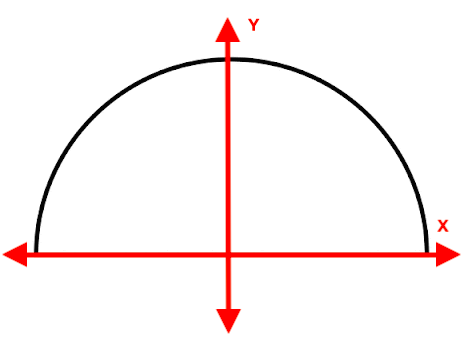
\includegraphics[scale=0.35]{P10}
	\centering
\end{figure}
Our dear, deer old friend center of mass integral has once again returned to haunt us. As can be seen from the diagram, I've oriented the semicircle such that it is symmetric about the y-axis, giving
\[ \boxed{ X_{COM} = 0} \]
To find the $Y_{COM}$, we will have to integrate. Let's recall the integral formula for Center of Mass
\begin{align}
	Y_{COM} &= \frac{ \int \rho y da}{\int \rho da} \\ 
	\intertext{Here $\rho$ is the density, it's uniform though so don't worry, it comes out of the integral and divides out. We'll also use $y = r\sin{\theta}$}
	&= \frac{ \int_0^R \int_0^{\pi} (r\sin{\theta}) rdrd\theta }{\int_0^R \int_0^{\pi} rdrd\theta} \\ 
	&= \frac{ \frac{R^3}{3}(2)}{\frac{\pi R^2}{2}} \\
	&= \frac{4R}{3\pi}
\end{align}
Our Center of Mass is therefore at \boxed{\left(0, \frac{4R}{3\pi}\right)} or $\approx 42\%$ of the way to the edge
%%%%%%%%%%%%%%%%% Problem 11 %%%%%%%%%%%%%%%%%
\section*{Problem 11} 
% Problem Statement
Show that the force $\vec{F}$ on a charge q due to a fixed charge Q at the origin is conservative and find the corresponding potential energy V.
%% Solution Here
\section*{\textit{Solution}} 
A conservative force is defined as one that is irrotational, or in math terms, that $\vcurl{F} = 0$
\begin{gather}
	\vec{F}_e = \frac{kQq}{r^2}\hat{r}  \\
	\intertext{Now we'll take the curl in spherical coordinates, check the back of Jackson or Wolfram for what this is, I can never remember}
	\vcurl{F}_e = \frac{1}{r\sin{\theta}} \left[\pdv{}{\theta}\left(F_{\phi}\sin{\theta}\right) - \pdv{}{\phi}F_{\theta}\right] \hat{r} + \frac{1}{r}\left[ \frac{1}{\sin{\theta}}\pdv{F_r}{\phi} - \pdv{}{r} (rF_{\phi})\right]\hat{\theta} + \frac{1}{r}\left[\pdv{}{r} (rF_{\theta}) - \pdv{}{\theta}F_r\right]\hat{\phi}
	\intertext{I wrote this all out so it's clear, but it will simplify very nicely if we examine (116)}
	F_{\theta} = F_{\phi} = 0 \\ 
	F_r(r) \Longrightarrow \dv{F_r}{\theta} = \dv{F_r}{\phi} = 0 \\ 
	\intertext{From (118) and (119) we see that ALL of the terms in (117) go away}
	\boxed{\vcurl{F} = 0 \text{ and so $\vec{F}$ is conservative as was to be proven}} 
\end{gather}
Next we are asked to find the potential associated with this. You might be able to remember this from E\&M, but it's never bad to just calculate it again for ourselves
\begin{align}
	\vec{F} &= -\vec{\nabla}V \\ 
	\int \vec{F} &= -\int \vec{\nabla}V \\ 
	\int \frac{kQq}{r^2}\hat{r} \cdot dr &= V \\ 
	\Aboxed{ \frac{kQq}{r} &= V(r), \text{as expected}}
\end{align}
%%%%%%%%%%%%%%%%% Problem 12 %%%%%%%%%%%%%%%%%
\section*{Problem 12} 
% Problem Statement
A small coin is placed on the top of frictionless sphere of radius R. The coin is given a tiny push and begins to slide down the sphere. At what vertical distance below the top of the sphere does the coin leave the surface of the sphere?
%% Solution Here
\begin{figure}[h]
	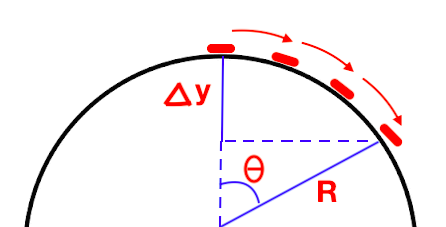
\includegraphics[scale=0.35]{P12}
	\centering
\end{figure}
\section*{\textit{Solution}} 
Hopefully the diagram above makes sense. We are trying to find the vertical distance at which the coin loses contact with the surface. The easiest way to do this will be to work in polar coordinates, then covert back at the end to cartesian. I believe there's a way to do this one with a Lagrangian, however conservation of energy should work just fine. \\
\\
\begin{align}
	\intertext{Let's start by defining what we are solving for}
	\Delta y &= y_f - y_i \\ 
	\Delta y &= R\cos{\theta} - R \\ 
	\Delta y &= -R(1 - \cos{\theta}) 
	\intertext{And now let's apply conservation of energy, with only kinetic and gravitational potential to worry about, we should have...}
	E_i = E_f \hspace{1cm}\Longrightarrow& \hspace{1cm}mgh_i = \frac{1}{2}mv^2 + mgh_f \\
	-\frac{1}{2}mv^2 &= mgh_f  - mgh_i \\ 
	 &= mg\Delta h \\
	 &= mg\Delta y \\ 
	 &= -mgR(1 - \cos{\theta}) \\ 
	v^2 &= 2gR(1 - \cos{\theta})
	\intertext{Alright, that's nice and juicy, let's think about Forces now. Before the coin falls off, it is exhibiting circular motion, so its acceleration will be centripetal}
	\Sigma F = ma_c &= \frac{mv^2}{R} \\ 
	\Sigma F = F_g &= mg\cos{\theta} \\
	v^2 &= Rg\cos{\theta} 
	\intertext{Where in (136), we combined (134) and (135). Now we'll substitute this definition of $v^2$ in (133)}
	2gR(1 - \cos{\theta}) &= Rg\cos{\theta} \\ 
	2 - 2\cos{\theta} &= \cos{\theta} \\ 
	2 &= 3\cos{\theta} \\ 
	\cos{\theta} &= \frac{2}{3}
	\intertext{We can take this result from (140) and combine it with (127) now}
	\Delta y &= -R(1 - \frac{2}{3}) \\ 
	\Aboxed{\Delta y &= \frac{-R}{3}}
\end{align}
So when the coin has slid one-third of the radius down, it will lose contact with the surface of the sphere. The negative sign is just because we're measuring distance \underline{from the top} of the sphere
%%%%%%%%%%%%%%%%% Problem 13 %%%%%%%%%%%%%%%%%
\section*{Problem13 } 
% Problem Statement
Consider a mass m moving in two dimensions with potential energy $V(x,y)=k(x^2+y^2)/2,k>0$. In the Cartesian (x,y) coordinate system, write down the Lagrangian and derive the two Lagrange equations of motion. Describe the solutions of the equations of motion
%% Solution Here
\section*{\textit{Solution}} 
\begin{align}
	\intertext{We're given the potential, so let's get right after the Lagrangian}
	\Lagr = T - V &= \fhalf m(\dot{x}^2 \dot{y}^2) - \frac{k(x^2+y^2)}{2}
	\intertext{Quick refresher on the general form of Euler-Lagrange Equations}
	\EulLagreq \\
	\text{Do x variable first }\rightarrow \hspace{3cm} \Aboxed{m\ddot{x} &= -kx} \\ 
	\text{Now y variable }\rightarrow \hspace{3cm} \Aboxed{m\ddot{y} &= -ky}
\end{align}
You probably recognize these differential equations, because they represent simple harmonic motion! They are solved by sin() and cos() functions
%%%%%%%%%%%%%%%%% Problem 14 %%%%%%%%%%%%%%%%%
\section*{Problem 14} 
% Problem Statement
A mass $m$ is attached by a massless string of length $l$ to the tip of a frictionless cone with vertex half-angle $\theta$. For the case when the mass moves at speed $v$ in a horizontal circle on the surface of the cone, find:
\begin{enumerate}[label=\alph*)]
	\item % PART (A)
	The tension in the string
	\item % PART (B)
	The nornal force on the mass from the cone
	\item % PART (C)
	The maximum speed $v$ for which the mass stays in contact with the cone
\end{enumerate}
\begin{figure}[h]
	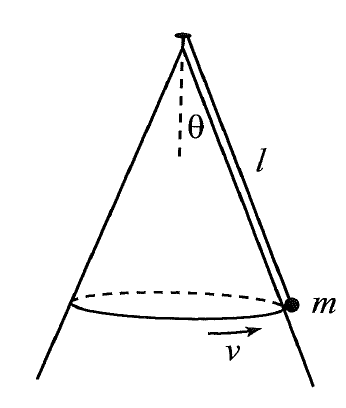
\includegraphics[scale=0.30]{P14_setup}
	\centering
\end{figure}
\begin{figure}[h]
	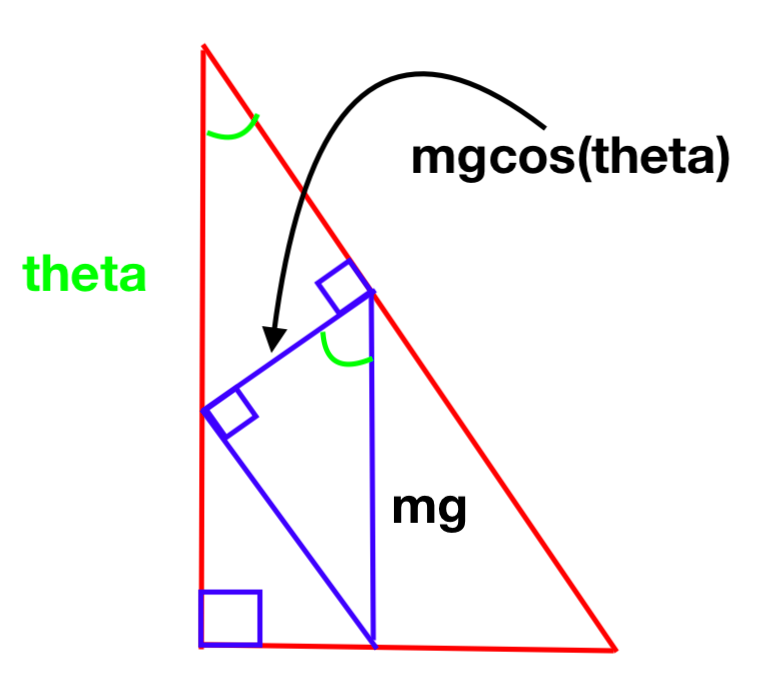
\includegraphics[scale=0.30]{P14_coords}
	\centering
\end{figure}
\begin{figure}[h]
	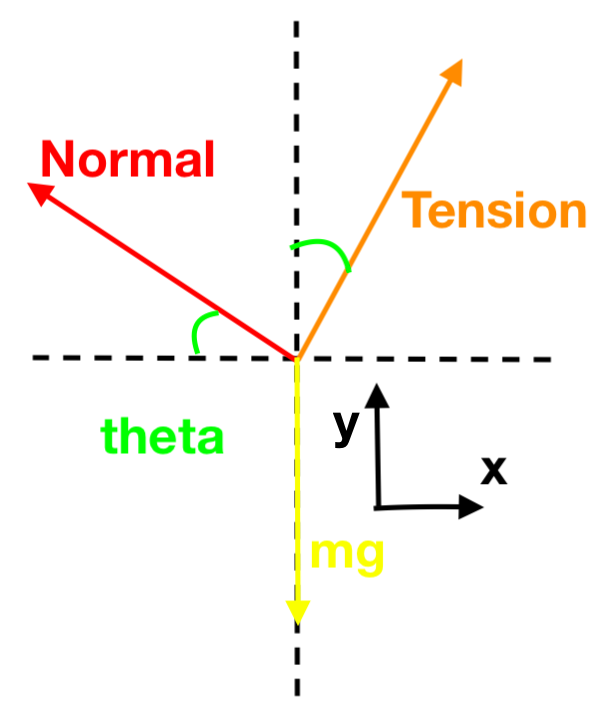
\includegraphics[scale=0.30]{P14_FBD}
	\centering
\end{figure}

%% Solution Here
\section*{\textit{Solution}} 
Ok, super weird situation, hopefully the following diagrams help visualize what in the world is going on. I chose not to use Lagrange approach for this and kinda just stuck with components and force analysis. For the rest of this problem, I'm also going to define my axis such that x is \underline{in to} the cone and y is \underline{straight up}. This will make things easier (I hope) \\ 
\\
Note: This is a variation on the Conical Pendulum problem, which there are lots of resources for \href{https://en.wikipedia.org/wiki/Conical_pendulum}{(Wiki Link)}. Basically just that with an added normal force, so if none of this is making sense (which it didn't to me), try to work through that simpler problem first, and then add a little spice
\begin{enumerate}[label=\alph*)]
	\item % PART (A)
	I'm gonna do (a) and (b) kinda together, just how it came out when I did this. Alrighty, the first thing to notice is that because the mass is traveling in a circular path, it will have centripetal acceleration
	\begin{align}
	\Sigma F_x &= ma_c = \frac{mv^2}{r} \\ 
	\Sigma F_x &= F_{Tx} + F_{Nx} = T\sin{\theta} - N\cos{\theta} \\
	&= T\sin{\theta} - N\cos{\theta} \\
	\Sigma F_y &= 0 = F_{Ty} + F_{gy} + F_{Ny} =  T\cos{\theta} + N\sin{\theta} - mg \\ 
	&=  T\cos{\theta} + N\sin{\theta} - mg \\ 
	T\cos{\theta} + N\sin{\theta} &= mg \\
	\intertext{Let's also get the radius r in terms of something better, and combine (147) with (149)}
	r &= l\sinth \\ 
	T\sin{\theta} - N\cos{\theta} &= \frac{mv^2}{l\sinth}\\ 
	\intertext{Now we can solve for T and yeet it in to (152), then follow the yellow brick road and solve for N}
	T &= \frac{mv^2}{l\sin^2{\theta}} + N\cot{\theta} \\ 
	mg &= \left( \frac{mv^2}{l\sin^2{\theta}} + N\frac{\costh}{\sinth}\right)\costh + N\sinth \\ 
	\intertext{Now we're going to divide both sides by $\costh$, for reasons that will become obvious (I hate when people do this)}
	\frac{mg}{\costh} &= \frac{mv^2}{l\sin^2{\theta}} + N\frac{\costh}{\sinth} + N\tan{\theta} \\ 
	\frac{mg}{\costh} &= \frac{mv^2}{l\sin^2{\theta}} + N\cot{\theta} + N\tan{\theta} \\
	\frac{mg}{\costh} &= \frac{mv^2}{l\sin^2{\theta}} + N(\cot{\theta} + \tan{\theta}) \\ 
	\intertext{There's a handy little Trig Identity that will help us now, getting close!}
	\cotth + \tanth &= \cscth \secth = \frac{1}{\costh \sinth} \\
	\frac{mg}{\costh} &= \frac{mv^2}{l\sin^2{\theta}} + \frac{N}{\costh \sinth} \\
	N &= \costh \sinth \left( \frac{mg}{\costh} - \frac{mv^2}{l\sin^2{\theta}} \right) \\
	\Aboxed{ N &= mg\sinth - \frac{mv^2}{l}\left( \frac{\costh}{\sinth} \right)} \\
	\intertext{So this is actually the answer to (b), oops, but for (a) all we need to do it take (164) and plug it in to (155), then solve for T, which I'll do right now :) }
	T &= \frac{mv^2}{l\sin^2{\theta}} + \left( mg\sinth - \frac{mv^2}{l}\frac{\costh}{\sinth} \right) \cot{\theta} \\
	T &= \frac{mv^2}{l\sin^2{\theta}} + mg\sinth \left( \frac{\costh}{\sinth} \right) - \frac{mv^2}{l} \left( \frac{\cos^2{\theta}}{\sin^2{\theta}} \right) \\
	T &= \frac{mv^2}{l\sin^2{\theta}} - \frac{mv^2}{l\sin^2{\theta}} \left( \cos^2{\theta}\right) + mg\sinth \left( \frac{\costh}{\sinth} \right) \\ 
	T &= \frac{mv^2}{l\sin^2{\theta}} \left(1 - \cos^2{\theta} \right) + mg\costh  \\ 
	\intertext{Now let's use a more familiar Trig Identity, $1 - \cos^2{\theta} = \sin^2{\theta}$}
	T &= \frac{mv^2}{l\sin^2{\theta}} \left(\sin^2{\theta} \right) + mg\costh \\
	\Aboxed{T &= \frac{mv^2}{l} + mg\costh}
	\end{align}
So we arrived at them out of order, but I think if you solve (154) for N, then yeet it in to (152), you'll get Tension first for (a). Either way, most of the work is in setting this up, then the two trig identities. 
	\item % PART (B)
	Just reproducing the result here for easy access
	\boxed{ N = mg\sinth - \frac{mv^2}{l}\left( \frac{\costh}{\sinth} \right)} 
	\item % PART (C)
	Ugh, somehow we have more to do. Alright, so for the maximum velocity before lifting off, that will be at the moment when the Normal Force equals zero, because the cone no longer has to push back on the mass at all. So let's start by setting the result from (b) equal to zero and solving for $v$
	\begin{align}
		mg\sinth - \frac{mv^2}{l}\left( \frac{\costh}{\sinth} \right) &= 0 \\
		\frac{mv^2}{l}\left( \frac{\costh}{\sinth} \right) &= mg\sinth \\ 
		v^2 &= \frac{gl\sin^2{\theta}}{\costh} \\
		\Aboxed{v &= \sqrt{ \frac{gl\sin^2{\theta}}{\costh} } }
	\end{align}
And here we've arrived at the maximum velocity, looks pretty nice, I'm surprised!
\end{enumerate}
%%%%%%%%%%%%%%%%% Problem 15 %%%%%%%%%%%%%%%%%
\section*{Problem 15} 
% Problem Statement
A pendulum bob of mass m is suspended by a massless spring (of unextended length l) with spring constant k. Derive the Lagrangian equations of motion.
\begin{figure}[h]
	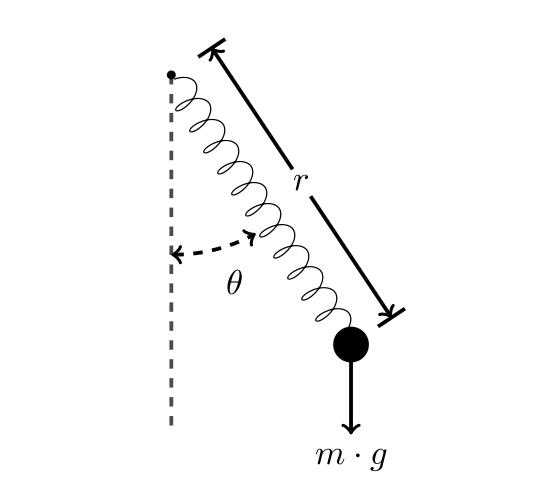
\includegraphics[scale=0.30]{P15}
	\centering
\end{figure}
%% Solution Here
\section*{\textit{Solution}} 
Alright, alright, alright... most of the work in this is in setting up the coordinate system and then writing out the Lagrangian. After that we have smooth sailing on the Euler-Lagrange Express \\ 
\\
Note: There are lots of good resources on this, just search for Elastic Pendulum, here's the \href{https://en.wikipedia.org/wiki/Elastic_pendulum}{Wiki Link} \\ 
\\
For our coordinates, we're going have an x-direction that is radially outwards, so along the spring, and a $\theta$-direction which is angular, in the direction the mass is swinging back and forth. You can call the x-direction the r-direction, not sure why I chose x but here we are
\begin{align}
	\Lagr &= T - V \\
	\intertext{For the Kinetic term, we have one linear term and one angular term}
	T &= \fhalf m\dot{x}^2 + \fhalf m x^2 \dot{\theta}^2
	\intertext{And for the Potential term, we have to account for the gravitational potential as well as the spring potential}
	V &= -mgx\costh + \fhalf k(x - l)^2
	\intertext{The gravity term we had to use a little trig, and the spring term is set up so that if $x=l$, and is therefore unstretched, there will be no potential energy, as expected}
	\Lagr &= \fhalf m\dot{x}^2 + \fhalf m x^2 \dot{\theta}^2 + mgx\costh - \fhalf k(x - l)^2 \\
	\EulLagreq \\
	\intertext{Now we can start taking derivatives, all aboard!!!}
	 m\ddot{x} &= mx\dot{\theta}^2 + mg\costh - k(x - l) \\ 
	 \Aboxed{\ddot{x} &= x\dot{\theta}^2 + g\costh - \frac{k}{m}(x - l) }\\
	 \intertext{Got the x equation of motion, now for $\theta$}
	mx^2\ddot{\theta} + 2m\dot{x}x\dot{\theta} &= - mgx\sinth \\
	mx^2\ddot{\theta} &= -2m\dot{x}x\dot{\theta} - mgx\sinth \\ 
	\Aboxed{\ddot{\theta} &= \frac{-2\dot{x}\dot{\theta}}{x} - \frac{g\sinth}{x}}
\end{align}
I apologize for doing this a little differently than the Wiki, if you use $x = x_w + l$, where $x_w$ is Wikipedia's x variable, you can see that it's the same. They used x as the distance from equilibrium, whereas I chose to make it the absolute radial distance from the hinge, just use whichever makes more sense to you
%%%%%%%%%%%%%%%%% Problem 16%%%%%%%%%%%%%%%%%
\section*{Problem 16} 
% Problem Statement
After a lengthy space flight, you have just landed on Planet X. Near the point where you are standing on the surface of Planet X, the gravitational force on a mass $m$ is vertically down but has a magnitude of $m\gamma y^2$, where $\gamma$ is a constant and y is the mass's height above the horizontal ground
\begin{enumerate}[label=\alph*)]
	\item % PART (A)
	Find the work done by gravity on a mass m moving from $\textbf{r}_1$ to $\textbf{r}_2$, and use your answer to show that gravity on Planet X, although most unusual, is still conservative
	\item % PART (B)
	Still on the same planet, you thread a bead on a curved, frictionless, rigid wire, which extends from ground level to a height $h$ above the ground. Show clearly the forces on the bead when it is somewhere on the wire. (Just name the forces so it is clear what they are; don't worry about their magnitude.) Which of the forces are conservative and which are not?
	\item % PART (C)
	If you release the bead from rest at height $h$, how fast will it be going when it reaches the ground?
\end{enumerate}
%% Solution Here
\section*{\textit{Solution}} 
What a weird problem. There are a couple different schools of thought on this one, and I honestly think if you explain your answer confidently, you'd get most credit. 
\begin{enumerate}[label=\alph*)]
	\item % PART (A)
	Ok, for a force to be conservative, it can't be path-dependent. That means that the work done is the same moving from one point to another, regardless of how we got there. So first, we'll find the work from $\vec{r}_1$ to $\vec{r}_2$
	\begin{align}
	\Delta W &= \int \vec{F}\cdot d\vec{l} \\ 
	&= \int_{\vec{r}_1}^{\vec{r}_2} m\gamma y^2 dy \\
	&= \frac{m\gamma}{3}(\vec{r}_2 - \vec{r}_1)
	\end{align}
From this, we can see that if $\vec{r}_1 = \vec{r}_2$, $\Delta W = 0$. This means our force is conservative. And if that wasn't good enough for you, try taking the curl of $\vec{F}$
	\begin{align}
	\vec{F} &= m\gamma y^2 \hat{y} \\ 
	\vcurl{F} &= \left(\pdv{F_z}{y} - \pdv{F_y}{z} \right) - \left( \pdv{F_z}{x} - \pdv{F_x}{z} \right) + \left( \pdv{F_y}{x} - \pdv{F_x}{y} \right) \\
	F_x = F_y &= \pdv{F_y}{x} = \pdv{F_y}{z} = 0 \\ 
	\vcurl{F} &= 0 
	\end{align}	
A conservative force by definition is irrotational
	\item % PART (B)
	Here's where things get dicey. We are asked to list the forces and state whether or not they are conservative. I've included a Free Body Diagram of how I picture this weird bead on a wire situation
	\begin{figure}[h]
	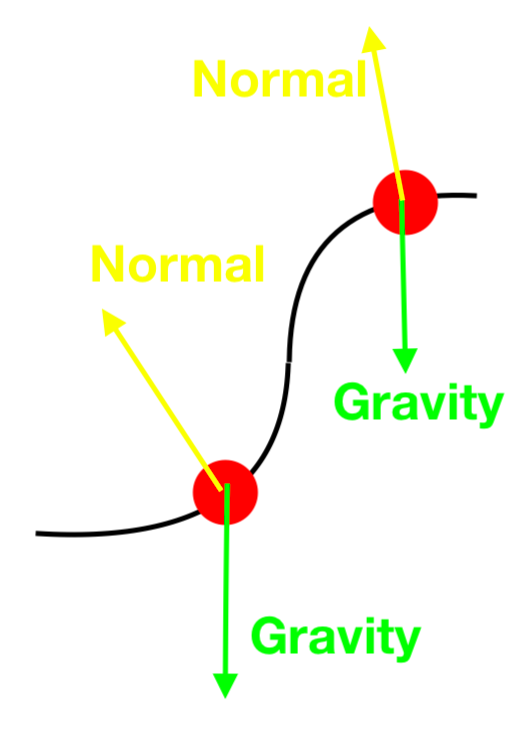
\includegraphics[scale=0.30]{P16}
	\centering
	\end{figure}
	From what I can see, there are only 2 forces: Gravity acting down always, and a Normal Force acting perpendicular to the wire (or perpendicular to the tangent of the curve). If the bead is traveling in a circular motion, then these forces could act like a centripetal force, but I don't think that just tells us what form $F=ma$ will take, and is not a separate force, ya dig?
	\begin{itemize}
		\item
		$F_g$: Gravitational Force is conservative, as proved in (A)
		\item
		$F_N$: Normal Force is also conservative, because it is built from $F_g$
	\end{itemize}
	\item % PART(C)
	Ok, now for some speeeeed. There's probably a Lagrangian approach for this, but let's not be too spicy and just do our normal conservation of energy
	\begin{align}
		V_i + T_i &= V_f + T_f \\ 
		h\cdot F_g + 0 &= 0 + \fhalf mv^2 \\ 
		h(m\gamma y^2) &= \fhalf mv^2 \\ 
		h(\gamma h^2 &= \fhalf v^2 \\
		v^2 &= 2\gamma h^3 \\
		v &= \sqrt{2\gamma h^3}
	\end{align}
\end{enumerate}

%%%%%%%%%%%%%%%%% Problem 17 %%%%%%%%%%%%%%%%%
\section*{Problem 17} 
% Problem Statement
\begin{enumerate}[label=\alph*)]
	\item % PART (A)
\end{enumerate}
%% Solution Here
\section*{\textit{Solution}} 
\begin{enumerate}[label=\alph*)]
	\item % PART (A)
\end{enumerate}

%%%%%%%%%%%%%%%%% Problem %%%%%%%%%%%%%%%%%
\section*{Problem } 
% Problem Statement
\begin{enumerate}[label=\alph*)]
	\item % PART (A)
\end{enumerate}
%% Solution Here
\section*{\textit{Solution}} 
\begin{enumerate}[label=\alph*)]
	\item % PART (A)
\end{enumerate}

%%%%%%%%%%%%%%%%% Problem %%%%%%%%%%%%%%%%%
\section*{Problem } 
% Problem Statement
\begin{enumerate}[label=\alph*)]
	\item % PART (A)
\end{enumerate}
%% Solution Here
\section*{\textit{Solution}} 
\begin{enumerate}[label=\alph*)]
	\item % PART (A)
\end{enumerate}

\end{document}





